%*============================================================*
%**Goal		:    文献分享:消失的女性与茶叶的价格
%**Author	:  	 ZhangYi zhangyiceee@163.com 15592606739
%**Created	:  	 20200323
%**Last Modified: 2020
%*============================================================*



\documentclass{beamer}
\usepackage[UTF8,noindent]{ctexcap}
\usepackage{natbib}
\usepackage{hyperref}


\graphicspath{{figures/}}




\usetheme{Madrid}
%\usecolortheme{crane} %黄色
%\usecolortheme{wolverine} %黄蓝
\usecolortheme{lily} %蓝白
%\usecolortheme{beetle} %灰色
%Information to be included in the title page:
\title[文献分享:ZY]{Malnutrition in early life and adult mental health: Evidence from a natural experiment}
\author[Huang et.al]{Huang et.al}
\date{\today}

\begin{document}

\frame{\titlepage}
%开始你的表演



%第1页幻灯片
%==========================================
\begin{frame}
\frametitle{Abstract}
饥荒是一次独特的机会来研究早期经历饥荒对于心理健康的影响,利用中国4972个出生在1956-1963年间的样本。
\\ we investigated the potential impact of exposure to the 1959e1961 Chinese Famine in utero and during the early postnatal life on adult mental illness.
\\ 结果发现与对照组相比出生在1959-1961年的女性有更高的GHQ(General Health Questionnaire)得分,并且提高了患有精神疾病的风险,饥荒时期出生的男性有耕地的GHQ得分,切患有精神疾病的风险与对照组相比不显著.
\\ 我们推测,早年遭受饥荒的长期后果包括选择最顽强的人和饥荒对幸存者的持久有害影响。在严重饥荒期间,男性胎儿与女性胎儿在子宫内的生物脆弱性更大,自然选择也更强,这可能会导致男性比女性有更强的选择效应,从而掩盖了饥荒对男性日后患精神疾病风险的有害影响

\end{frame}

\begin{frame}
\frametitle{文献的贡献}
	分性别来看影响
\end{frame}


\begin{frame}
\frametitle{结果}
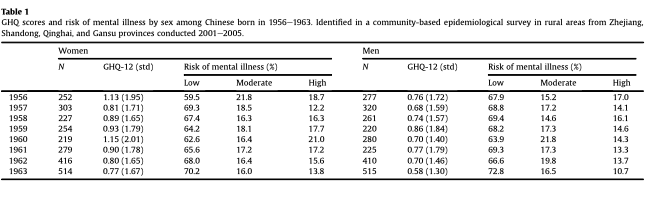
\includegraphics[scale=0.5]{table1}
每个地区的饥荒程度有所不同,因此需要构造饥荒严重程度的指数。
\end{frame}

\begin{frame}
\frametitle{衡量饥荒严重程度}
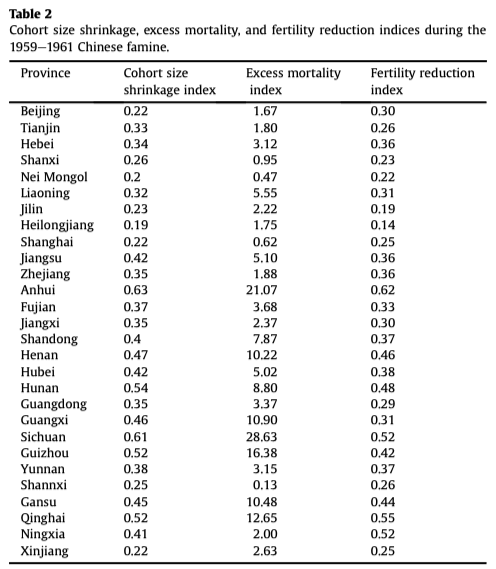
\includegraphics[scale=0.5]{table2}
	
\end{frame}

\begin{frame}
\frametitle{结果}
\centering{
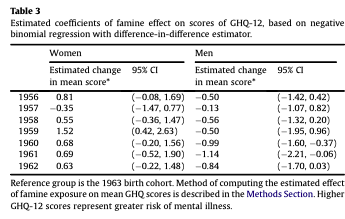
\includegraphics[scale=0.5]{table3}
	
只对1959年出生的有显著影响} 
\end{frame}

\begin{frame}
\frametitle{}
	
\end{frame}

\begin{frame}
\frametitle{}
	
\end{frame}

%参考文献的案例 \citet{Krueger1999Experimental} \citep{Krueger1999Experimental}  注意两类的不同
\end{document}



